\chapter{Függvények használata}
\thispagestyle{empty}

\section{Függvények beszúrása}

A függvények jelentősen megkönnyítik a számítási és
egyéb feladatok elvégzését a táblázatkezelő
programokban.

A függvények két részből állnak: a függvény
nevéből és argumentumból. Az argumentumot zárójelek
között kell megadnunk. Egy függvénynek több argumentuma is
lehet, ilyenkor pontosvesszővel választjuk el őket
egymástól. A függvény általános alakja tehát:
\begin{center}
=FÜGGVÉNYNÉV(argumentum1; argumentum2; ...)
\end{center}

Van olyan függvény is, amelynek nincs argumentuma, a zárójeleket
ilyenkor sem hagyhatjuk el. Például a matematikában használatos
${\pi}$ számot meg tudjuk adni cellában függvénnyel: =PI().

A leggyakrabban használt függvény a SZUM, ami összeadja az
argumentumlistájában lévő számokat. A SZUM függvény a
következő argumentummal =SZUM(A1:A4;C2) egyenértékű az
$=A1+A2+A3+A4+C2$ képlettel. Ezen az egyszerű példán is
láthatjuk, hogy a függvények használata megkönnyíti a
számításokat.

Függvényeket a \textbf{Beszúrás} menüpont
\textbf{Függvény} parancsával (Ctrl+F2) vagy a \textbf{Képlet}
eszköztár ikonjaival hozhatunk létre. Ezek közül az első
a \textbf{Függvénytündér}, a második az \textbf{Összeg}
és a harmadik a \textbf{Függvény}.

\begin{figure}[!h]
\begin{center}
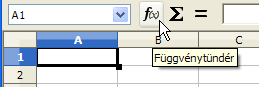
\includegraphics[width=7.751cm]{oocalcv2-img32.png}
\caption{Függvénytündér}\label{Függvénytündér}
\end{center}
\end{figure}

A \textbf{Függvény} ikon (\aref{Függvénytündér} ábrán az
,,='' feliratú) megkönnyíti a
legutóbb használt függvények ismételt kiválasztását
(\ref{FüggvényKiválasztás} ábra).
Nagyon hasznos funkció, hiszen a Calc több száz
függvénye közül egy munkalapon rendszerint csak néhányat
használunk. 

\begin{figure}[h]
\begin{center}
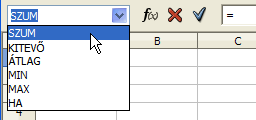
\includegraphics[width=5.772cm]{oocalcv2-img33.png}
\caption{Függvény kiválasztása}\label{FüggvényKiválasztás}
\end{center}
\end{figure}

\Aref{FüggvényKiválasztás} ábrán látható, hogy az eszköztár ikonjai is
megváltoztak: megjelent a \textbf{Mégse} és az
\textbf{Elfogadás} parancs. Ezekkel, egér segítségével is
nyugtázhatjuk a kiválasztott függvényeket és argumentumokat.

\section{Egyszerűbb statisztikai függvények használata}
(SZUM, MIN, MAX, ÁTLAG, DARAB, DARAB2, KICSI, NAGY)

A Calc program magyar nyelvű változatában általában magyar
függvénynevekkel találkozunk.\footnote{A OpenOffice.org 3.2.1-es 
verziótól kezdve} Ezek a magyar függvénynevek megegyeznek a magyar
Excelben lévőkkel. Csak azok a függvénynevek 
nincsenek lefordítva, amelyek nem léteznek a magyar Excelben, 
vagy abban nincsenek lefordítva. Ezeknek az angolul maradt 
függvényeknek a használata az angol
nyelvet nem ismerők számára sem jelenthet gondot, hiszen a
függvények magyarázata és a súgó példái magyar nyelvűek. 

A Calc súgója megkönnyíti azok dolgát, aki csak az angol függvényneveket
ismerik. A magyar megfelelő kikereséséhez válasszuk a Súgó
ablakában a \textbf{Tárgymutató}t, a \textbf{Keresett
kifejezés}hez pedig írjuk a függvény angol nevét
(\ref{SúgóÁtlag} ábra).


\begin{figure}[!h]
\begin{center}
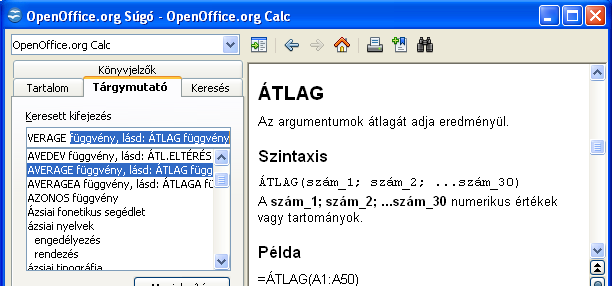
\includegraphics[width=13.193cm]{oocalcv2-img34.png}
\caption{OpenOffice.org Súgó --  Átlag}\label{SúgóÁtlag}
\end{center}
\end{figure}

\Aref{AlapvetőFüggvények} táblázatban a négy leggyakrabban használt
függvényt láthatjuk.

\begin{table}[!h]
\begin{center}
\caption{Alapvető függvények}\label{AlapvetőFüggvények}
\begin{tabular}{|m{2.5cm}|m{8cm}|m{3cm}|}
\hline
\multicolumn{1}{|c|}{\textbf{A függvény}}&
\multicolumn{1}{c|}{\textbf{Funkciója}}&
\multicolumn{1}{c|}{\textbf{A függvény}} \\
\multicolumn{1}{|c|}{\textbf{neve}} & &
\multicolumn{1}{c|}{\textbf{angol neve}} \\
\hline
SZUM & Összeadja a cellatartományban lévő számokat. & SUM \\
\hline
MIN & Az argumentumlista legkisebb értékét adja eredményül. & MIN \\
\hline
MAX & Az argumentumlista legnagyobb értékét adja eredményül. & MAX \\   
\hline
ÁTLAG & Az argumentumok átlagát adja eredményül. & AVERAGE \\
\hline
\end{tabular}
\end{center}
\end{table}

A Függvénytündér használatának begyakorlására
készítsük el a következő feladatot.


\section{7. feladat}

{\itshape
Másoljuk egy üres munkafüzetbe a \textbf{ZH 02} munkalapot. A
munkalapon töröljük a képlettel kiszámított cellák
tartalmát. Számítsuk ki az összpontszámokat a G oszlopban a
SZUM függvénnyel. A 8. sorban függvény segítségével
jelenítsük meg a feladatok és az összpontszámok átlagát.
 Határozzuk meg a legnagyobb és a legkisebb összpontszámot,
valamint azt, hogy a legtöbb  pontszámot elért tanulónak
hány pont hiányzik a maximálisan elérhetőhöz. Mentsük a
munkafüzetet \textbf{calc02} néven.}

A munkalap tartalmát átmásolhatjuk kijelölve, másolva és a
másik munkafüzetbe beillesztve azt, de gyorsabb módszer a
munkafüzet beszúrása (\textbf{Beszúrás} menüpont
\textbf{Munkalap} parancs). Itt válasszuk a \textbf{Fájlból}
kapcsolót, majd a \textbf{Tallózás} parancs segítségével
adjuk meg annak a munkafüzetnek a  nevét, amelyik a szükséges
munkalapot tartalmazza (\ref{7-feladatMunkalap} ábra).

\begin{figure}[!h]
\begin{center}
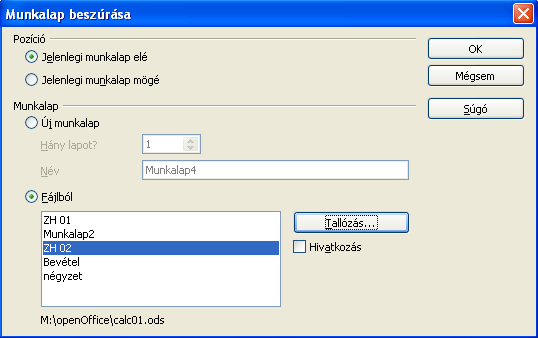
\includegraphics[width=11.235cm]{oocalcv2-img35.png}
\caption{7. feladat --  Munkafüzet beszúrása}\label{7-feladatMunkalap}
\end{center}
\end{figure}

Jelöljük ki a ZH 02 munkalap nevét és szúrjuk be az aktuális
munkafüzetünkbe.
A munkalapon jelöljük ki a G4:G7 tartományt és a
,,Backspace'' billentyűvel
töröljük a tartalmát. 

\begin{figure}[!h]
\begin{center}
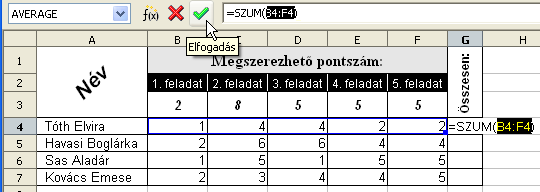
\includegraphics[width=11.288cm]{oocalcv2-img36.png}
\caption{7. feladat}\label{7-feladat}
\end{center}
\end{figure}

Tegyük aktívvá a G4 cellát és kattintsunk a \textbf{Képlet}
eszköztár \textbf{Összeg} ikonjára. A cellában megjelenik a
SZUM függvény és a megfelelő argumentumok is. A Calc az
aktív cellától balra egy számsort talált és azt beírta a
SZUM függvénybe argumentumként. Ez nagyon hasznos funkció,
hiszen gyakran fordul elő, hogy egy sor végén, vagy egy oszlop
alján kell annak összegét kiszámolni. A kék színű keret
 mutatja az automatikusan meghatározott tartományt (\ref{7-feladat} ábra).

A képletet három cellán át lefelé másolva megkapjuk mind a
négy tanuló összpontszámát.

Az A8 cellába írjuk az ,,Átlag''
szót és a B8 cellában válasszuk a függvénytündért 
(\ref{7-feladatFüggvény} ábra).

\begin{figure}[!h]
\begin{center}
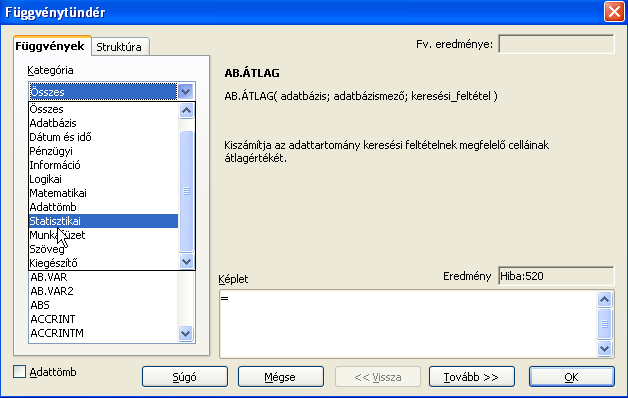
\includegraphics[width=13.999cm]{oocalcv2-img37.png}
\caption{7. feladat --  függvénytündér}\label{7-feladatFüggvény}
\end{center}
\end{figure}

\begin{figure}[!h]
\begin{center}
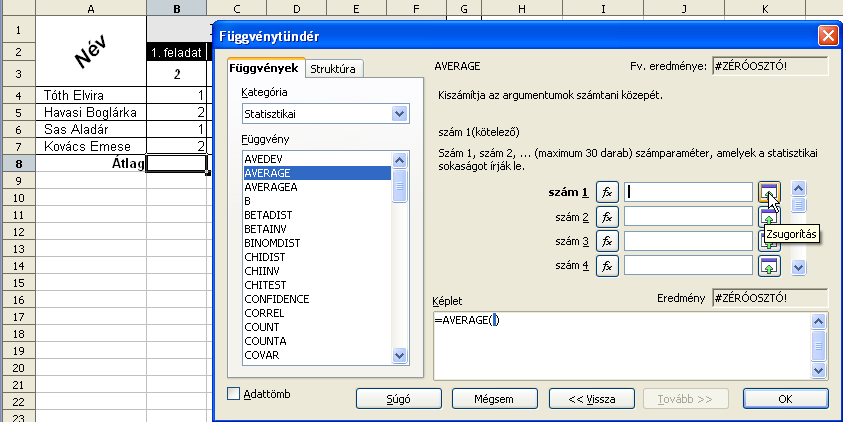
\includegraphics[width=15.999cm]{oocalcv2-img38.png}
\caption{7. feladat }\label{7-feladatArgumentum}
\end{center}
\end{figure}

Az ablakban kategóriákba rendezetten találjuk a Calc összes
függvényét. Egy függvényt kiválasztva az ablak jobb
oldalán annak a magyarázatát olvashatjuk. A \textbf{Statisztikai}
kategóriából válasszuk az ÁTLAG függvényt. A
\textbf{Tovább} gombra kattintva a párbeszédablak jobb oldalán
megjelennek az argumentumbeviteli mezők (\ref{7-feladatArgumentum} ábra).
Jelöljük ki a B4:B7 tartományt és a cellahivatkozás megjelenik az első
beviteli mezőben. Természetesen megadhatunk szám- és egyéb
értékeket, illetve hivatkozásokat a párbeszédablak megfelelő részeiben.  

A \textbf{Zsugorítás} ikon lecsökkenti a párbeszédablakot a
beviteli mező méretére. Így könnyebb a szükséges
hivatkozást megjelölni a lapon. Az ikon ezután automatikusan
átalakul a \textbf{Maximalizálás} ikonra. Erre kattintva a
párbeszédablakot visszaállíthatjuk eredeti méretére.

Bonyolultabb függvények esetén hasznos lehet a \textbf{Súgó}
parancs. A megjelenő ablakban részletes leírást és
példákat olvashatunk a kiválasztott függvényről.

Másoljuk a függvénytündérrel létrehozott B8 cellát jobbra
minden feladat és a csoport összpontszám átlagának
kiszámításához.

A legtöbb és a legkevesebb összpontszámot jelenítsük meg a
B11 és B10 cellákban a MAX és MIN függvények
segítségével. A B12 cella azt a pontszámot mutatja, amennyivel
kevesebbet ért el a legjobb tanuló az elérhető maximumnál.
Ennek kiszámításához is használhatjuk a
függvénytündért az első függvény megadása után, a
 mínusz jelet beírva a Képlet párbeszédablakba és megadva
a második függvényt (\ref{7-feladatMásodik} ábra).

\begin{figure}[!h]
\begin{center}
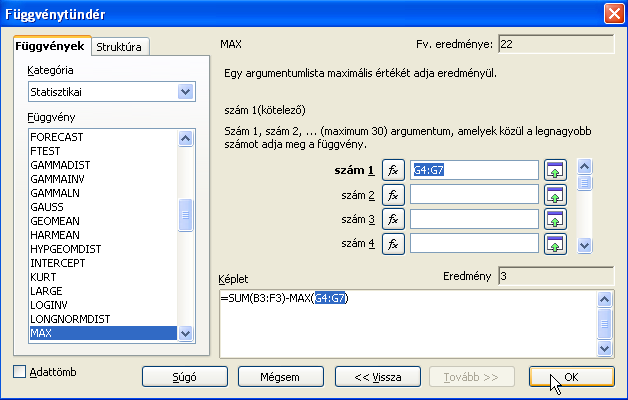
\includegraphics[width=15.999cm]{oocalcv2-img39.png}
\caption{ 7. feladat}\label{7-feladatMásodik}
\end{center}
\end{figure}

Amennyiben pontosan ismerjük a használni kívánt függvény
szintaxisát, nem kell feltétlenül használnunk a
függvénytündért, a cellába közvetlenül is beírhatjuk a
kifejezést.

\clearpage
Az elkészült feladat \aref{7-feladatMegoldás} ábrán látható.

A következő feladatban \aref{StatisztikaiFüggvények} táblázatban
felsorolt statisztikai függvényeket fogjuk használni.

\begin{figure}[!h]
\begin{center}
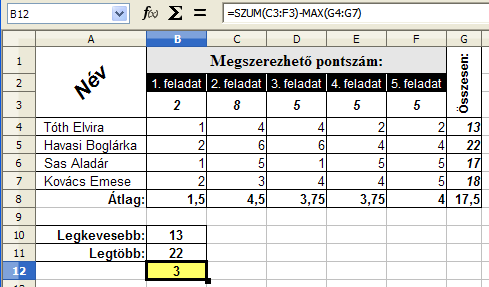
\includegraphics[width=14.936cm]{oocalcv2-img40.png}
\caption{7. feladat}\label{7-feladatMegoldás}
\end{center}
\end{figure}

\begin{table}[!h]
\begin{center}
\caption{Statisztikai függvények}\label{StatisztikaiFüggvények}
\begin{tabular}{|m{2.5cm}|m{8cm}|m{3cm}|}
\hline
\multicolumn{1}{|c|}{\textbf{A függvény}}&
\multicolumn{1}{c|}{\textbf{Funkciója}}&
\multicolumn{1}{c|}{\textbf{A függvény}} \\
\multicolumn{1}{|c|}{\textbf{neve}} & &
\multicolumn{1}{c|}{\textbf{angol neve}} \\
\hline
DARAB &
Megszámolja, hány szám van a paraméterlistában. A szöveges
bejegyzéseket kihagyja. &
COUNT\\ \hline
DARAB2 &
Megszámolja, hány érték van a paraméterlistában. A
szöveges elemek is számítanak. &
COUNTA\\ \hline
KICSI &
Kiszámítja egy adathalmaz $k$-adik legkisebb értékét. &
SMALL\\ \hline
NAGY &
Kiszámítja egy adathalmaz $k$-adik legnagyobb értékét. &
LARGE\\ \hline
\end{tabular}
\end{center}
\end{table}

\section{8. feladat}

{\itshape
\Aref{8-feladat} ábrán egy iskolai futóverseny eredményeit látjuk. Hozzuk
létre a calc02 munkafüzet második munkalapján az alábbi
táblázatot. A D oszlopban jelenjen meg a tanulók jobbik
eredménye. A G oszlop számadatait függvény segítségével
számítsuk ki.}

\begin{figure}[!h]
\begin{center}
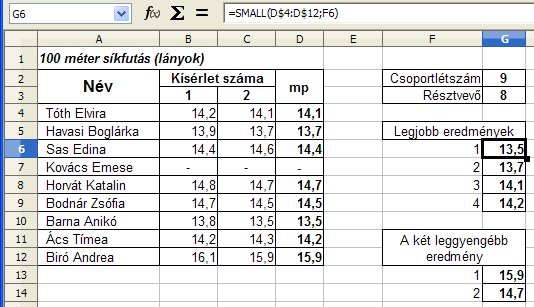
\includegraphics[width=14.125cm]{oocalcv2-img41.png}
\caption{8. feladat}\label{8-feladat}
\end{center}
\end{figure}

A csoportlétszámot a DARAB2 függvénnyel, a résztvevők
számát pedig a DARAB-bal számíthatjuk ki. Az argumentumlista
lehet ugyanaz (D4:D12), hiszen a DARAB csak a számokat tartalmazó
cellák darabszámát adja meg.

A KICSI függvénnyel meghatározhatjuk egy cellatartomány $k$-adik
legkisebb értékét. Két kötelező paramétere van: az
elsővel a tartományt adjuk meg, a másodikkal meghatározzuk,
hogy hányadik legkisebb elemre van szükségünk. Figyeljük meg
\aref{8-feladat} ábrán, hogy ez a paraméter relatív cellahivatkozás
(F6). A képlet másolásakor ez az argumentum a megfelelő
értéket fogja felvenni. Az első paraméternél viszont vegyes
cellahivatkozást használunk, hogy minden másolt függvény
ugyanarra  a tartományra hivatkozzon.

A G13:G14 tartományt hasonlóan számítjuk ki, csak itt a NAGY
függvényt alkalmazva.

